% Designs
\section{Power Calculations}
\begin{table}[!htb]
  \centering
  \renewcommand{\arraystretch}{1.2}
  \begin{tabular}{ |c|c|c|c| }
  \hline
  \textbf{Component}        & \textbf{Voltage}    & \textbf{Current}     & \textbf{Power}   \\
  \hline
  Motors                    & 24 V                & 0.5 A (x4)           & 48 W             \\ \hline
  Motor Drivers             & 5 V                 & 89 mA (x2)           & 890 mW           \\ \hline
  ESP32 Dev Board           & 5 V                 & 120 mA               & 660 mW           \\ \hline
  RA-02                     & 3.3 V               & 100 mA               & 330 mW           \\ \hline
  ATGM332D-5N31             & 3.3 V               & 25 mA                & 82.5 mW          \\ \hline
  MPU-9250                  & 3.3 V               & 3.7 mA               & 12.21 mW         \\ \hline
  \textbf{Total}            &                     &                      & \textbf{49.97 W}         \\ \hline
  \end{tabular}
  \caption{Ground Station Total Power Calculation}
  \label{tab:gs_component_consumption}
\end{table}

\begin{table}[!htb]
  \centering
  \renewcommand{\arraystretch}{1.2}
  \begin{tabular}{ |c|c|c| }
  \hline
  \textbf{Component}        & \textbf{Current}        & \textbf{Power (@ 3V3)}      \\ \hline 
  ATmega328                 & 12 mA                   & 39.6 mW                     \\ \hline 
  RA-02                     & 100 mA                  & 330 mW                      \\ \hline 
  ATGM332D-5N31             & 25 mA                   & 82.5 mW                     \\ \hline
  MAX485                    & 137.3 mA                & 1.0 mW                        \\ \hline
  \textbf{Total}            &                         & \textbf{453.1 mW}         \\ \hline
  \end{tabular}
  \caption{PocketQube Unit Component Power Consumption}
  \label{tab:pqunit_component_consumption}
\end{table}


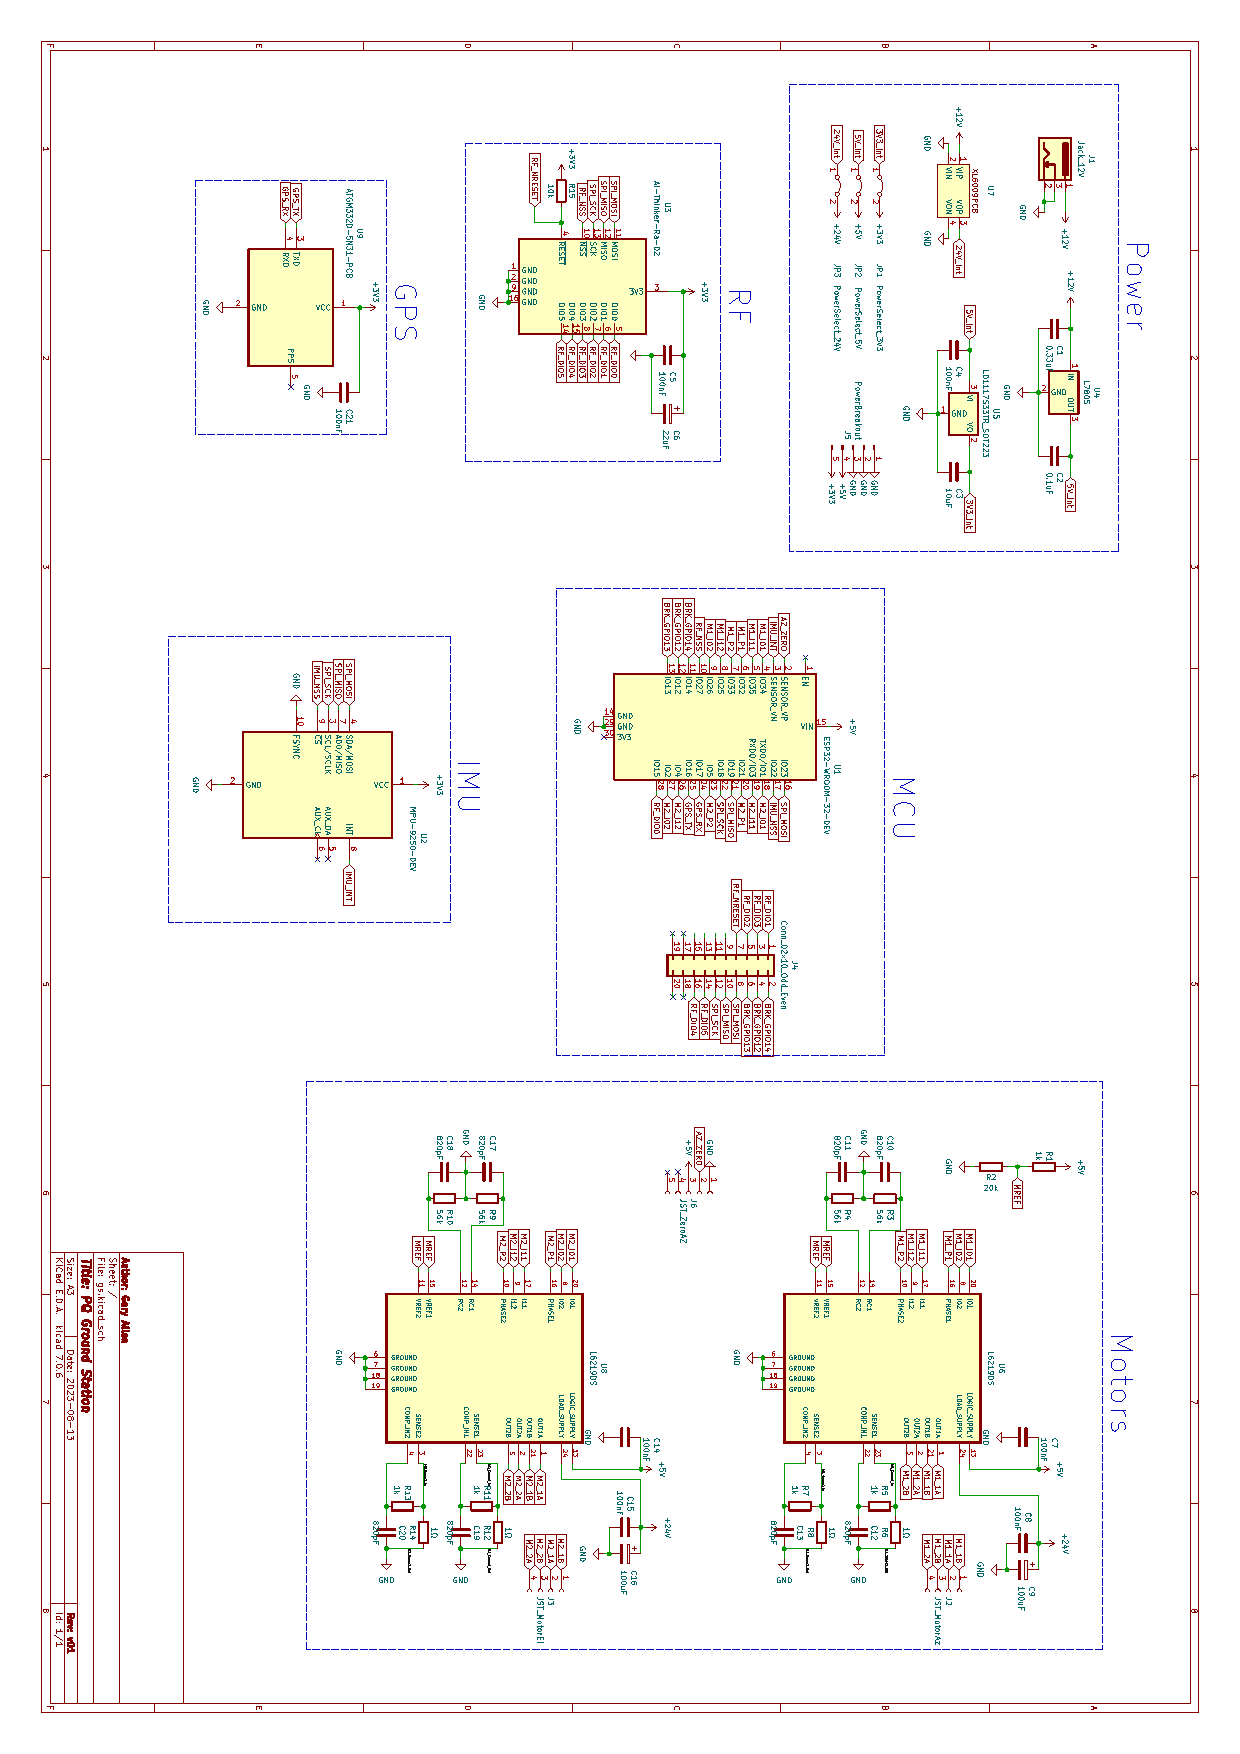
\includepdf[scale=0.65,pages=1,offset=0mm -35mm,pagecommand=\chapter{Design}\section{Ground Station Schematic}\label{sec:appendix_gs_schematics}]{docs/gs_schematic}
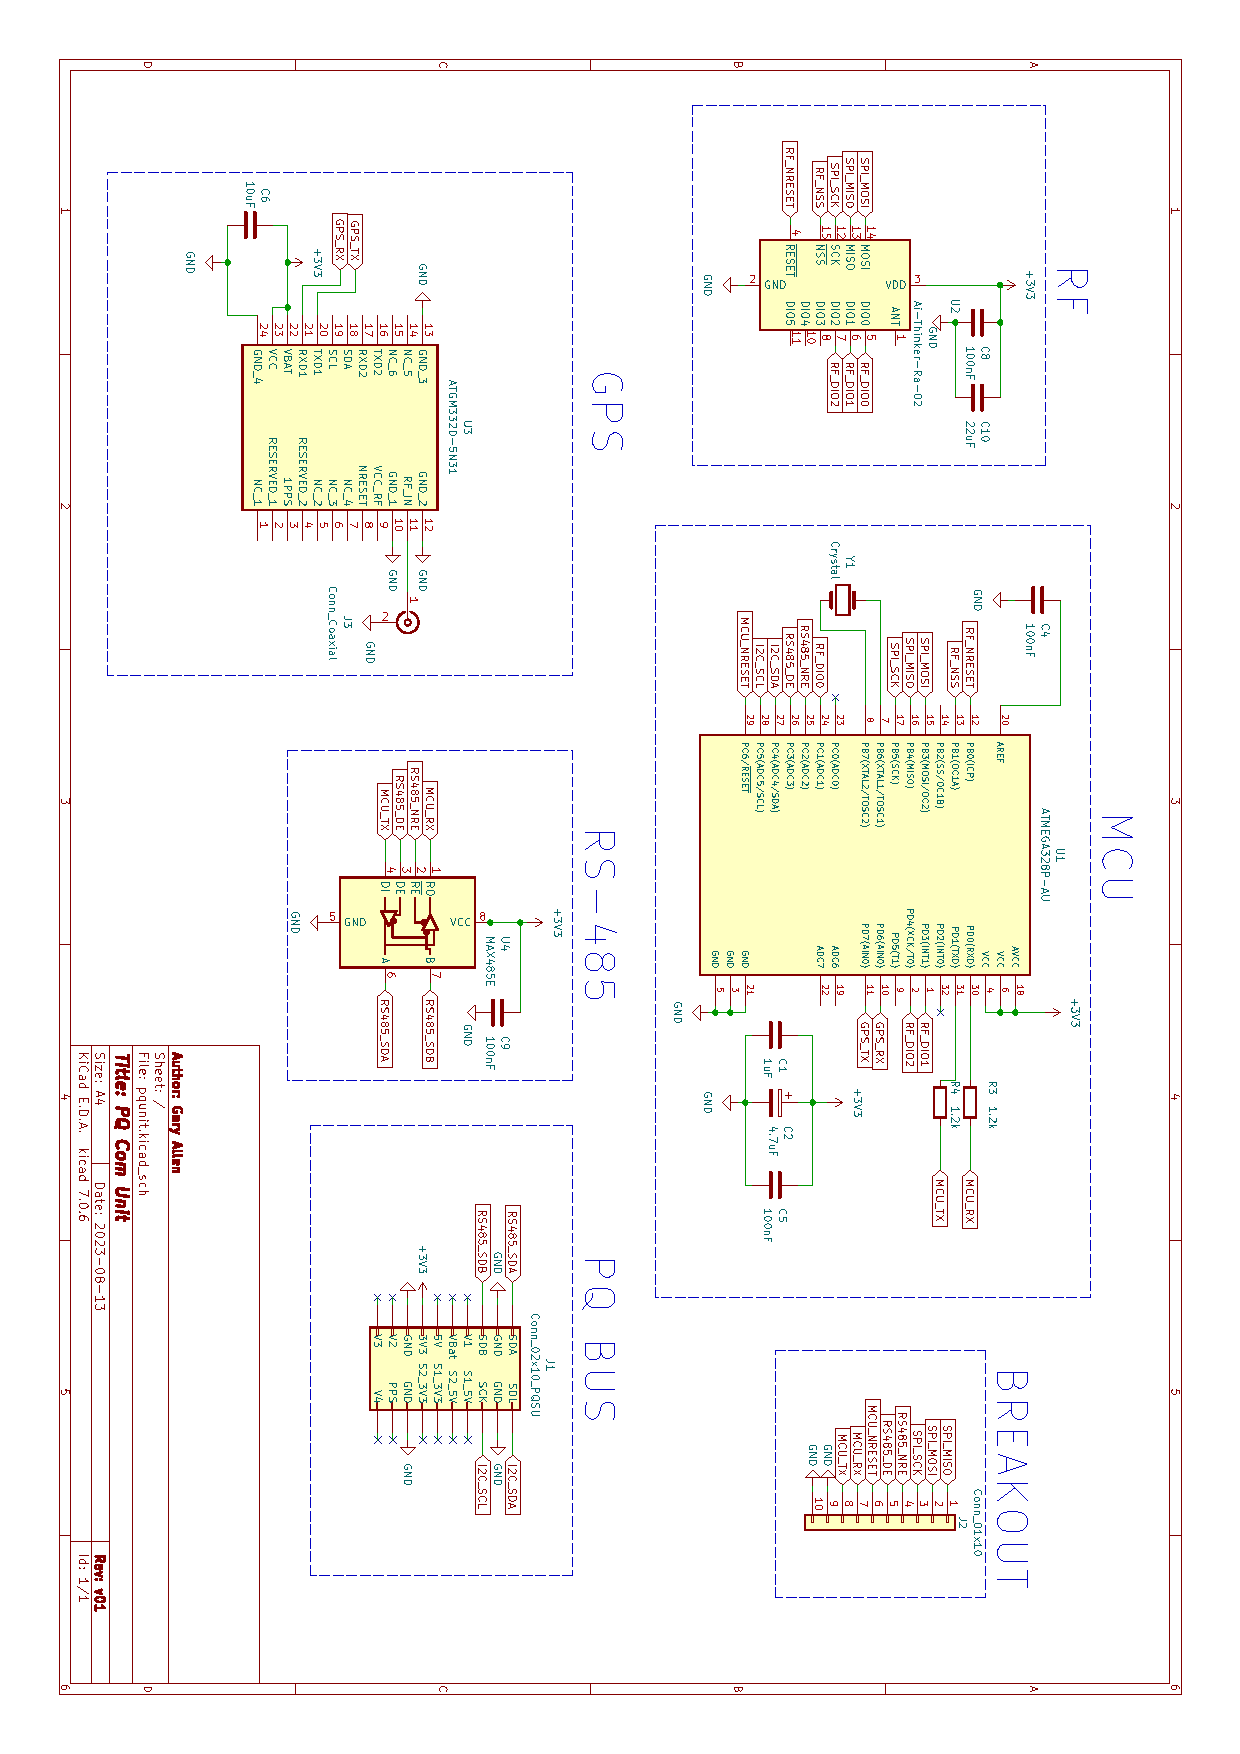
\includepdf[scale=0.7,pages=1,pagecommand=\section{PocketQube Unit Schematic}\label{sec:appendix_pq_schematic}]{docs/pq_schematic}

\section{Ground Station PCB}\label{sec:appendix_gs_pcb_design}
\begin{figure}[!htb]
  \centering
  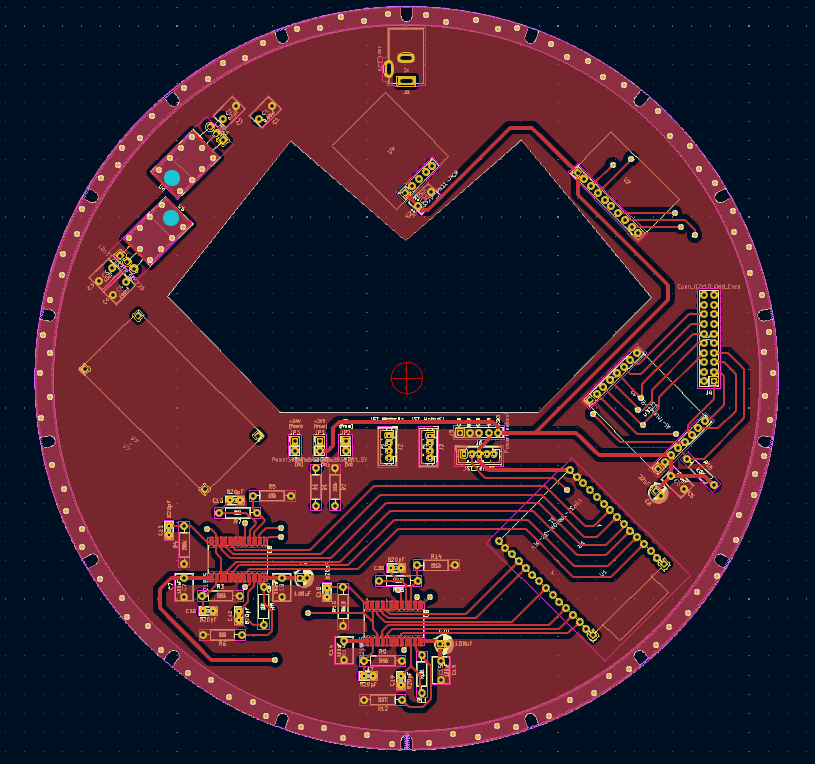
\includegraphics[width=0.6\textwidth]{gs_pcb_design}
  \caption{Ground Station PCB Design}
  \label{fig:gs_pcb}
\end{figure}

\section{PCB Errata}\label{sec:appendix_pcb_errata}
Ground Station PCB:
% \itemi

\section{Ground Station Antenna}
\begin{table}[!htb]
  \centering
  \renewcommand{\arraystretch}{1.2}
  \begin{tabular}{ |c|c| }
  \hline
  \textbf{Parameter}                  & \textbf{Value}    \\
  \hline
  Diameter (D)                        & 187.1 mm          \\ \hline
  Turn Spacing (S)                    & 88.2 mm           \\ \hline
  No. of Turns (n)                    & 4                 \\ \hline
  Ground plane diameter (G)           & $> \SI{350}{mm}$  \\ \hline
  Strip height (sh)                   & 19.4 mm          \\ \hline
  Strip width (sw)                    & 77.7 mm           \\ \hline
  Strip length (sl)                   & 132 mm           \\ \hline
  Cup height, if used (ch)            & 88.2 mm           \\ \hline
  \end{tabular}
  \caption{Helical Antenna Final Parameters}
  \label{tab:helicalParameters}
\end{table}

\section{Software}
\begin{table}[!htb]
  \centering
  \caption{GPS Class}
  \renewcommand{\arraystretch}{1.2}
  \begin{tabular}{ |c|c| }
  \hline
  \textbf{Function}        & \textbf{Description}    \\
  \hline
    getLocation()              & Return latitude, longitude and altitude \\
    getTime()                  & Return seconds since epoch \\
  \hline
  \end{tabular}
  \label{tab:gpsUML}
\end{table}

\begin{table}[!htb]
  \centering
  \caption{Radio Class}
  \renewcommand{\arraystretch}{1.2}
  \begin{tabular}{ |c|c| }
  \hline
  \textbf{Function}        & \textbf{Description}    \\
  \hline
    startTransmit(message)              & Transmit data (non-blocking i.e. with callback) \\
    startReceive()                      & Start listening to receive data (non-blocking i.e. with callback) \\
    getRssi()                           & Get signal strength \\
    getSnr()                            & Get signal-to-noise ratio \\
  \hline
  \end{tabular}
  \label{tab:radioUML}
\end{table}

\begin{table}[!htb]
  \centering
  \caption{Link Class}
  \renewcommand{\arraystretch}{1.2}
  \begin{tabular}{ |c|c| }
  \hline
  \textbf{Function}        & \textbf{Description}    \\
  \hline
  setTelemetryCallback(fn)                    & Set the "telemetry sent/received" function  \\
  setTelecommandCallback(fn)                  & Set the "telecommand received" function (\textit{Responder} only) \\
  \hline
  \end{tabular}
  \label{tab:linkUML}
\end{table}

\begin{table}[!htb]
  \centering
  \caption{StepperMotor Class}
  \renewcommand{\arraystretch}{1.2}
  \begin{tabular}{ |c|c| }
  \hline
  \textbf{Function}        & \textbf{Description}    \\
  \hline
    stepForward(numSteps)         & Blocking and non-blocking options \\
    saveZeroPosition()            & Used for calibration \\
    getPosition()                 & Used for open-loop feedback \\
    setSpeed()                    & Sets the delay between steps \\
    setCurrentMultiplier()        & Set the amount of current \\
  \hline
  \end{tabular}
  \label{tab:stepperMotorUML}
\end{table}

\begin{table}[!htb]
  \centering
  \caption{Mount Class}
  \renewcommand{\arraystretch}{1.2}
  \begin{tabular}{ |c|c| }
  \hline
  \textbf{Function}        & \textbf{Description}    \\
  \hline
    calibrate()                         & Calbrate the mount \\
    setAzimuthalElevation(az, el)       & Set the azimuthal and elevation angles \\
    setBoresight(boresightVec)          & Set the boresight pointing vector \\
  \hline
  \end{tabular}
  \label{tab:mountUML}
\end{table}

\begin{table}[!htb]
  \centering
  \caption{GroundStation Class}
  \renewcommand{\arraystretch}{1.2}
  \begin{tabular}{ |c|c| }
  \hline
  \textbf{Function}             & \textbf{Description}    \\
  \hline
    calibrate()                 & Calibrate the entire GS \\
    addEstimatedLocation(loc)      & Add an estimated input GPS location for open-loop tracking \\
    addKnownLocation(loc)          & Add a known GPS location for closed-loop tracking \\
  \hline
  \end{tabular}
  \label{tab:groundStationUML}
\end{table}
